% Options for packages loaded elsewhere
% Options for packages loaded elsewhere
\PassOptionsToPackage{unicode}{hyperref}
\PassOptionsToPackage{hyphens}{url}
\PassOptionsToPackage{dvipsnames,svgnames,x11names}{xcolor}
%
\documentclass[
  letterpaper,
  DIV=11,
  numbers=noendperiod]{scrartcl}
\usepackage{xcolor}
\usepackage{amsmath,amssymb}
\setcounter{secnumdepth}{-\maxdimen} % remove section numbering
\usepackage{iftex}
\ifPDFTeX
  \usepackage[T1]{fontenc}
  \usepackage[utf8]{inputenc}
  \usepackage{textcomp} % provide euro and other symbols
\else % if luatex or xetex
  \usepackage{unicode-math} % this also loads fontspec
  \defaultfontfeatures{Scale=MatchLowercase}
  \defaultfontfeatures[\rmfamily]{Ligatures=TeX,Scale=1}
\fi
\usepackage{lmodern}
\ifPDFTeX\else
  % xetex/luatex font selection
\fi
% Use upquote if available, for straight quotes in verbatim environments
\IfFileExists{upquote.sty}{\usepackage{upquote}}{}
\IfFileExists{microtype.sty}{% use microtype if available
  \usepackage[]{microtype}
  \UseMicrotypeSet[protrusion]{basicmath} % disable protrusion for tt fonts
}{}
\makeatletter
\@ifundefined{KOMAClassName}{% if non-KOMA class
  \IfFileExists{parskip.sty}{%
    \usepackage{parskip}
  }{% else
    \setlength{\parindent}{0pt}
    \setlength{\parskip}{6pt plus 2pt minus 1pt}}
}{% if KOMA class
  \KOMAoptions{parskip=half}}
\makeatother
% Make \paragraph and \subparagraph free-standing
\makeatletter
\ifx\paragraph\undefined\else
  \let\oldparagraph\paragraph
  \renewcommand{\paragraph}{
    \@ifstar
      \xxxParagraphStar
      \xxxParagraphNoStar
  }
  \newcommand{\xxxParagraphStar}[1]{\oldparagraph*{#1}\mbox{}}
  \newcommand{\xxxParagraphNoStar}[1]{\oldparagraph{#1}\mbox{}}
\fi
\ifx\subparagraph\undefined\else
  \let\oldsubparagraph\subparagraph
  \renewcommand{\subparagraph}{
    \@ifstar
      \xxxSubParagraphStar
      \xxxSubParagraphNoStar
  }
  \newcommand{\xxxSubParagraphStar}[1]{\oldsubparagraph*{#1}\mbox{}}
  \newcommand{\xxxSubParagraphNoStar}[1]{\oldsubparagraph{#1}\mbox{}}
\fi
\makeatother

\usepackage{color}
\usepackage{fancyvrb}
\newcommand{\VerbBar}{|}
\newcommand{\VERB}{\Verb[commandchars=\\\{\}]}
\DefineVerbatimEnvironment{Highlighting}{Verbatim}{commandchars=\\\{\}}
% Add ',fontsize=\small' for more characters per line
\usepackage{framed}
\definecolor{shadecolor}{RGB}{241,243,245}
\newenvironment{Shaded}{\begin{snugshade}}{\end{snugshade}}
\newcommand{\AlertTok}[1]{\textcolor[rgb]{0.68,0.00,0.00}{#1}}
\newcommand{\AnnotationTok}[1]{\textcolor[rgb]{0.37,0.37,0.37}{#1}}
\newcommand{\AttributeTok}[1]{\textcolor[rgb]{0.40,0.45,0.13}{#1}}
\newcommand{\BaseNTok}[1]{\textcolor[rgb]{0.68,0.00,0.00}{#1}}
\newcommand{\BuiltInTok}[1]{\textcolor[rgb]{0.00,0.23,0.31}{#1}}
\newcommand{\CharTok}[1]{\textcolor[rgb]{0.13,0.47,0.30}{#1}}
\newcommand{\CommentTok}[1]{\textcolor[rgb]{0.37,0.37,0.37}{#1}}
\newcommand{\CommentVarTok}[1]{\textcolor[rgb]{0.37,0.37,0.37}{\textit{#1}}}
\newcommand{\ConstantTok}[1]{\textcolor[rgb]{0.56,0.35,0.01}{#1}}
\newcommand{\ControlFlowTok}[1]{\textcolor[rgb]{0.00,0.23,0.31}{\textbf{#1}}}
\newcommand{\DataTypeTok}[1]{\textcolor[rgb]{0.68,0.00,0.00}{#1}}
\newcommand{\DecValTok}[1]{\textcolor[rgb]{0.68,0.00,0.00}{#1}}
\newcommand{\DocumentationTok}[1]{\textcolor[rgb]{0.37,0.37,0.37}{\textit{#1}}}
\newcommand{\ErrorTok}[1]{\textcolor[rgb]{0.68,0.00,0.00}{#1}}
\newcommand{\ExtensionTok}[1]{\textcolor[rgb]{0.00,0.23,0.31}{#1}}
\newcommand{\FloatTok}[1]{\textcolor[rgb]{0.68,0.00,0.00}{#1}}
\newcommand{\FunctionTok}[1]{\textcolor[rgb]{0.28,0.35,0.67}{#1}}
\newcommand{\ImportTok}[1]{\textcolor[rgb]{0.00,0.46,0.62}{#1}}
\newcommand{\InformationTok}[1]{\textcolor[rgb]{0.37,0.37,0.37}{#1}}
\newcommand{\KeywordTok}[1]{\textcolor[rgb]{0.00,0.23,0.31}{\textbf{#1}}}
\newcommand{\NormalTok}[1]{\textcolor[rgb]{0.00,0.23,0.31}{#1}}
\newcommand{\OperatorTok}[1]{\textcolor[rgb]{0.37,0.37,0.37}{#1}}
\newcommand{\OtherTok}[1]{\textcolor[rgb]{0.00,0.23,0.31}{#1}}
\newcommand{\PreprocessorTok}[1]{\textcolor[rgb]{0.68,0.00,0.00}{#1}}
\newcommand{\RegionMarkerTok}[1]{\textcolor[rgb]{0.00,0.23,0.31}{#1}}
\newcommand{\SpecialCharTok}[1]{\textcolor[rgb]{0.37,0.37,0.37}{#1}}
\newcommand{\SpecialStringTok}[1]{\textcolor[rgb]{0.13,0.47,0.30}{#1}}
\newcommand{\StringTok}[1]{\textcolor[rgb]{0.13,0.47,0.30}{#1}}
\newcommand{\VariableTok}[1]{\textcolor[rgb]{0.07,0.07,0.07}{#1}}
\newcommand{\VerbatimStringTok}[1]{\textcolor[rgb]{0.13,0.47,0.30}{#1}}
\newcommand{\WarningTok}[1]{\textcolor[rgb]{0.37,0.37,0.37}{\textit{#1}}}

\usepackage{longtable,booktabs,array}
\usepackage{calc} % for calculating minipage widths
% Correct order of tables after \paragraph or \subparagraph
\usepackage{etoolbox}
\makeatletter
\patchcmd\longtable{\par}{\if@noskipsec\mbox{}\fi\par}{}{}
\makeatother
% Allow footnotes in longtable head/foot
\IfFileExists{footnotehyper.sty}{\usepackage{footnotehyper}}{\usepackage{footnote}}
\makesavenoteenv{longtable}
\usepackage{graphicx}
\makeatletter
\newsavebox\pandoc@box
\newcommand*\pandocbounded[1]{% scales image to fit in text height/width
  \sbox\pandoc@box{#1}%
  \Gscale@div\@tempa{\textheight}{\dimexpr\ht\pandoc@box+\dp\pandoc@box\relax}%
  \Gscale@div\@tempb{\linewidth}{\wd\pandoc@box}%
  \ifdim\@tempb\p@<\@tempa\p@\let\@tempa\@tempb\fi% select the smaller of both
  \ifdim\@tempa\p@<\p@\scalebox{\@tempa}{\usebox\pandoc@box}%
  \else\usebox{\pandoc@box}%
  \fi%
}
% Set default figure placement to htbp
\def\fps@figure{htbp}
\makeatother





\setlength{\emergencystretch}{3em} % prevent overfull lines

\providecommand{\tightlist}{%
  \setlength{\itemsep}{0pt}\setlength{\parskip}{0pt}}



 


\KOMAoption{captions}{tableheading}
\makeatletter
\@ifpackageloaded{caption}{}{\usepackage{caption}}
\AtBeginDocument{%
\ifdefined\contentsname
  \renewcommand*\contentsname{Table of contents}
\else
  \newcommand\contentsname{Table of contents}
\fi
\ifdefined\listfigurename
  \renewcommand*\listfigurename{List of Figures}
\else
  \newcommand\listfigurename{List of Figures}
\fi
\ifdefined\listtablename
  \renewcommand*\listtablename{List of Tables}
\else
  \newcommand\listtablename{List of Tables}
\fi
\ifdefined\figurename
  \renewcommand*\figurename{Figure}
\else
  \newcommand\figurename{Figure}
\fi
\ifdefined\tablename
  \renewcommand*\tablename{Table}
\else
  \newcommand\tablename{Table}
\fi
}
\@ifpackageloaded{float}{}{\usepackage{float}}
\floatstyle{ruled}
\@ifundefined{c@chapter}{\newfloat{codelisting}{h}{lop}}{\newfloat{codelisting}{h}{lop}[chapter]}
\floatname{codelisting}{Listing}
\newcommand*\listoflistings{\listof{codelisting}{List of Listings}}
\makeatother
\makeatletter
\makeatother
\makeatletter
\@ifpackageloaded{caption}{}{\usepackage{caption}}
\@ifpackageloaded{subcaption}{}{\usepackage{subcaption}}
\makeatother
\usepackage{bookmark}
\IfFileExists{xurl.sty}{\usepackage{xurl}}{} % add URL line breaks if available
\urlstyle{same}
\hypersetup{
  pdftitle={ST695\_SPD\_Analysis},
  colorlinks=true,
  linkcolor={blue},
  filecolor={Maroon},
  citecolor={Blue},
  urlcolor={Blue},
  pdfcreator={LaTeX via pandoc}}


\title{ST695\_SPD\_Analysis}
\author{}
\date{2025-09-29}
\begin{document}
\maketitle


\textbf{Instantiate Libraries}

\begin{Shaded}
\begin{Highlighting}[]
\FunctionTok{library}\NormalTok{(lmerTest) }\CommentTok{\#Needed for REML Analysis}
\end{Highlighting}
\end{Shaded}

\begin{verbatim}
Loading required package: lme4
\end{verbatim}

\begin{verbatim}
Loading required package: Matrix
\end{verbatim}

\begin{verbatim}

Attaching package: 'lmerTest'
\end{verbatim}

\begin{verbatim}
The following object is masked from 'package:lme4':

    lmer
\end{verbatim}

\begin{verbatim}
The following object is masked from 'package:stats':

    step
\end{verbatim}

\textbf{Import PLA Data}

\begin{Shaded}
\begin{Highlighting}[]
\NormalTok{Ys\_data }\OtherTok{\textless{}{-}} \FunctionTok{read.csv}\NormalTok{(}\StringTok{"Data/YsData.csv"}\NormalTok{)}
\NormalTok{Ys\_data }\OtherTok{\textless{}{-}}\NormalTok{ Ys\_data[,}\DecValTok{7}\SpecialCharTok{:}\DecValTok{13}\NormalTok{]}
\NormalTok{Ys\_data}\SpecialCharTok{$}\NormalTok{WP}\OtherTok{=}\FunctionTok{as.factor}\NormalTok{(Ys\_data}\SpecialCharTok{$}\NormalTok{WP)}
\FunctionTok{write.csv}\NormalTok{(Ys\_data, }\AttributeTok{file =} \StringTok{"Data/Ys\_Data\_Subset.csv"}\NormalTok{)}

\NormalTok{Yw\_data }\OtherTok{\textless{}{-}} \FunctionTok{read.csv}\NormalTok{(}\StringTok{"Data/YwData.csv"}\NormalTok{)}
\NormalTok{Yw\_data }\OtherTok{\textless{}{-}}\NormalTok{ Yw\_data[,}\DecValTok{14}\SpecialCharTok{:}\DecValTok{17}\NormalTok{]}
\FunctionTok{write.csv}\NormalTok{(Yw\_data, }\AttributeTok{file =} \StringTok{"Data/Yw\_Data\_Subset.csv"}\NormalTok{)}
\end{Highlighting}
\end{Shaded}

\textbf{Method 1 (Ordinary Least Squares)}

\begin{Shaded}
\begin{Highlighting}[]
\NormalTok{WP\_factors }\OtherTok{\textless{}{-}} \FunctionTok{colnames}\NormalTok{(Ys\_data[}\DecValTok{1}\SpecialCharTok{:}\DecValTok{3}\NormalTok{])}
\NormalTok{SP\_factors }\OtherTok{\textless{}{-}} \FunctionTok{colnames}\NormalTok{(Ys\_data[}\DecValTok{4}\SpecialCharTok{:}\DecValTok{5}\NormalTok{])}
\NormalTok{linear\_terms }\OtherTok{\textless{}{-}} \FunctionTok{c}\NormalTok{(WP\_factors, SP\_factors)}

\CommentTok{\# Model with all main effects and 2{-}way interactions}
\NormalTok{fo }\OtherTok{\textless{}{-}} \FunctionTok{as.formula}\NormalTok{(}
  \FunctionTok{paste}\NormalTok{(}
    \StringTok{"Denier \textasciitilde{} ("}\NormalTok{, }
    \FunctionTok{paste}\NormalTok{(linear\_terms, }\AttributeTok{collapse =} \StringTok{" + "}\NormalTok{), }
    \StringTok{")\^{}2"}
\NormalTok{  )}
\NormalTok{)}

\NormalTok{Method\_1 }\OtherTok{\textless{}{-}} \FunctionTok{summary}\NormalTok{(}\FunctionTok{lm}\NormalTok{(fo, }\AttributeTok{data =}\NormalTok{ Ys\_data))}
\NormalTok{Method\_1}
\end{Highlighting}
\end{Shaded}

\begin{verbatim}

Call:
lm(formula = fo, data = Ys_data)

Residuals:
    Min      1Q  Median      3Q     Max 
-62.225 -26.034  -0.719  27.928  58.100 

Coefficients:
             Estimate Std. Error t value Pr(>|t|)    
(Intercept)  299.0906     9.0640  32.998 2.03e-15 ***
T             -3.1156     9.0640  -0.344 0.735815    
P             98.4344     9.0640  10.860 1.67e-08 ***
S           -145.0969     9.0640 -16.008 7.72e-11 ***
D           -131.9031     9.0640 -14.552 2.97e-10 ***
R            -19.4969     9.0640  -2.151 0.048181 *  
T:P            0.2406     9.0640   0.027 0.979171    
T:S           -3.0781     9.0640  -0.340 0.738867    
T:D           -0.9719     9.0640  -0.107 0.916033    
T:R           -2.8156     9.0640  -0.311 0.760350    
P:S          -37.0906     9.0640  -4.092 0.000962 ***
P:D          -54.6844     9.0640  -6.033 2.29e-05 ***
P:R            0.3344     9.0640   0.037 0.971059    
S:D           86.8969     9.0640   9.587 8.68e-08 ***
S:R            2.9406     9.0640   0.324 0.750093    
D:R          -10.4156     9.0640  -1.149 0.268500    
---
Signif. codes:  0 '***' 0.001 '**' 0.01 '*' 0.05 '.' 0.1 ' ' 1

Residual standard error: 49.74 on 15 degrees of freedom
Multiple R-squared:  0.981, Adjusted R-squared:  0.9619 
F-statistic: 51.53 on 15 and 15 DF,  p-value: 3.718e-10
\end{verbatim}

Residual Standard Error: 49.74. Error variance estimate: 49.74\^{}2 =
2474.8

The error variance (mean squared error, MSE) is 2474.8 in your model.
This value is the estimate of the residual variance from your standard
linear model.

\textbf{Method 2 (Restricted Maximum Likelihood)}

\begin{Shaded}
\begin{Highlighting}[]
\NormalTok{WP\_factors }\OtherTok{\textless{}{-}} \FunctionTok{colnames}\NormalTok{(Ys\_data[}\DecValTok{1}\SpecialCharTok{:}\DecValTok{3}\NormalTok{])}
\NormalTok{SP\_factors }\OtherTok{\textless{}{-}} \FunctionTok{colnames}\NormalTok{(Ys\_data[}\DecValTok{4}\SpecialCharTok{:}\DecValTok{5}\NormalTok{])}

\NormalTok{linear\_terms }\OtherTok{\textless{}{-}} \FunctionTok{c}\NormalTok{(WP\_factors, SP\_factors)}

\CommentTok{\# Model with all main effects, 2{-}way interactions, and random WP effect}
\NormalTok{fo }\OtherTok{\textless{}{-}} \FunctionTok{as.formula}\NormalTok{(}
  \FunctionTok{paste}\NormalTok{(}
    \StringTok{"Denier \textasciitilde{} ("}\NormalTok{, }
    \FunctionTok{paste}\NormalTok{(linear\_terms, }\AttributeTok{collapse =} \StringTok{" + "}\NormalTok{), }
    \StringTok{")\^{}2 + (1|WP)"}
\NormalTok{  )}
\NormalTok{)}

\NormalTok{Method\_2 }\OtherTok{\textless{}{-}} \FunctionTok{summary}\NormalTok{(}\FunctionTok{lmer}\NormalTok{(fo, }\AttributeTok{data =}\NormalTok{ Ys\_data))}
\end{Highlighting}
\end{Shaded}

\begin{verbatim}
boundary (singular) fit: see help('isSingular')
\end{verbatim}

\begin{Shaded}
\begin{Highlighting}[]
\NormalTok{Method\_2}
\end{Highlighting}
\end{Shaded}

\begin{verbatim}
Linear mixed model fit by REML. t-tests use Satterthwaite's method [
lmerModLmerTest]
Formula: fo
   Data: Ys_data

REML criterion at convergence: 214.5

Scaled residuals: 
     Min       1Q   Median       3Q      Max 
-1.25093 -0.52338 -0.01445  0.56145  1.16801 

Random effects:
 Groups   Name        Variance Std.Dev.
 WP       (Intercept)    0      0.00   
 Residual             2474     49.74   
Number of obs: 31, groups:  WP, 8

Fixed effects:
             Estimate Std. Error        df t value Pr(>|t|)    
(Intercept)  299.0906     9.0640   15.0000  32.998 2.03e-15 ***
T             -3.1156     9.0640   15.0000  -0.344 0.735815    
P             98.4344     9.0640   15.0000  10.860 1.67e-08 ***
S           -145.0969     9.0640   15.0000 -16.008 7.72e-11 ***
D           -131.9031     9.0640   15.0000 -14.552 2.97e-10 ***
R            -19.4969     9.0640   15.0000  -2.151 0.048181 *  
T:P            0.2406     9.0640   15.0000   0.027 0.979171    
T:S           -3.0781     9.0640   15.0000  -0.340 0.738867    
T:D           -0.9719     9.0640   15.0000  -0.107 0.916033    
T:R           -2.8156     9.0640   15.0000  -0.311 0.760350    
P:S          -37.0906     9.0640   15.0000  -4.092 0.000962 ***
P:D          -54.6844     9.0640   15.0000  -6.033 2.29e-05 ***
P:R            0.3344     9.0640   15.0000   0.037 0.971059    
S:D           86.8969     9.0640   15.0000   9.587 8.68e-08 ***
S:R            2.9406     9.0640   15.0000   0.324 0.750093    
D:R          -10.4156     9.0640   15.0000  -1.149 0.268500    
---
Signif. codes:  0 '***' 0.001 '**' 0.01 '*' 0.05 '.' 0.1 ' ' 1
\end{verbatim}

\begin{verbatim}

Correlation matrix not shown by default, as p = 16 > 12.
Use print(x, correlation=TRUE)  or
    vcov(x)        if you need it
\end{verbatim}

\begin{verbatim}
optimizer (nloptwrap) convergence code: 0 (OK)
boundary (singular) fit: see help('isSingular')
\end{verbatim}

\textbf{Method 4 ANOVA}

\begin{Shaded}
\begin{Highlighting}[]
\NormalTok{WP\_factors }\OtherTok{\textless{}{-}} \FunctionTok{colnames}\NormalTok{(Ys\_data[}\DecValTok{1}\SpecialCharTok{:}\DecValTok{3}\NormalTok{])}
\NormalTok{SP\_factors }\OtherTok{\textless{}{-}} \FunctionTok{colnames}\NormalTok{(Ys\_data[}\DecValTok{4}\SpecialCharTok{:}\DecValTok{5}\NormalTok{])}
\NormalTok{linear\_terms }\OtherTok{\textless{}{-}} \FunctionTok{c}\NormalTok{(WP\_factors, SP\_factors)}

\CommentTok{\# Model with all main effects, 2{-}way interactions,}
\CommentTok{\#and split{-}plot error structure}

\NormalTok{fo }\OtherTok{\textless{}{-}} \FunctionTok{as.formula}\NormalTok{(}
  \FunctionTok{paste}\NormalTok{(}
    \StringTok{"Denier \textasciitilde{} ("}\NormalTok{, }
    \FunctionTok{paste}\NormalTok{(linear\_terms, }\AttributeTok{collapse =} \StringTok{" + "}\NormalTok{), }
    \StringTok{")\^{}2 + Error(WP)"}
\NormalTok{  )}
\NormalTok{)}

\NormalTok{Method\_4\_ANOVA }\OtherTok{\textless{}{-}} \FunctionTok{summary}\NormalTok{(}\FunctionTok{aov}\NormalTok{(fo, }\AttributeTok{data =}\NormalTok{ Ys\_data))}
\NormalTok{Method\_4\_ANOVA}
\end{Highlighting}
\end{Shaded}

\begin{verbatim}

Error: WP
    Df Sum Sq Mean Sq
T    1   2251    2251
P    1 356982  356982
S    1 613959  613959
D    1  23273   23273
T:P  1   2808    2808
T:S  1   9591    9591
P:S  1  23020   23020

Error: Within
          Df Sum Sq Mean Sq F value   Pr(>F)    
D          1 527529  527529 199.115 1.14e-09 ***
R          1  13710   13710   5.175   0.0392 *  
T:D        1     16      16   0.006   0.9388    
T:R        1    685     685   0.259   0.6190    
P:D        1 107948  107948  40.745 1.70e-05 ***
P:R        1    927     927   0.350   0.5635    
S:D        1 226165  226165  85.366 2.47e-07 ***
S:R        1    377     377   0.142   0.7116    
D:R        1   3290    3290   1.242   0.2839    
Residuals 14  37091    2649                     
---
Signif. codes:  0 '***' 0.001 '**' 0.01 '*' 0.05 '.' 0.1 ' ' 1
\end{verbatim}

\textbf{Method 5A Additional Replicates}

\begin{Shaded}
\begin{Highlighting}[]
\CommentTok{\# Function to simulate whole{-}plot and sub{-}plot replicates}
\NormalTok{WP\_SP\_replicates }\OtherTok{\textless{}{-}} \ControlFlowTok{function}\NormalTok{(data, }\AttributeTok{response =} \StringTok{"Denier"}\NormalTok{, }\AttributeTok{r =} \DecValTok{3}\NormalTok{, }\AttributeTok{sd =} \DecValTok{5}\NormalTok{, }\AttributeTok{seed =} \DecValTok{123}\NormalTok{) \{}
  \FunctionTok{set.seed}\NormalTok{(seed)}
  \CommentTok{\# Repeat each row r times}
\NormalTok{  data\_rep }\OtherTok{\textless{}{-}}\NormalTok{ data[}\FunctionTok{rep}\NormalTok{(}\DecValTok{1}\SpecialCharTok{:}\FunctionTok{nrow}\NormalTok{(data), }\AttributeTok{each =}\NormalTok{ r), ]}
  \CommentTok{\# Add replicate identifier}
\NormalTok{  data\_rep}\SpecialCharTok{$}\NormalTok{RPL }\OtherTok{\textless{}{-}} \FunctionTok{rep}\NormalTok{(}\DecValTok{1}\SpecialCharTok{:}\NormalTok{r, }\AttributeTok{times =} \FunctionTok{nrow}\NormalTok{(data))}
  \CommentTok{\# Add random noise to the response variable}
\NormalTok{  data\_rep[[response]] }\OtherTok{\textless{}{-}}\NormalTok{ data\_rep[[response]] }\SpecialCharTok{+} \FunctionTok{rnorm}\NormalTok{(}\FunctionTok{nrow}\NormalTok{(data\_rep), }\AttributeTok{mean =} \DecValTok{0}\NormalTok{, }\AttributeTok{sd =}\NormalTok{ sd)}
  \FunctionTok{rownames}\NormalTok{(data\_rep) }\OtherTok{\textless{}{-}} \ConstantTok{NULL}
  \FunctionTok{return}\NormalTok{(data\_rep)}
\NormalTok{\}}

\CommentTok{\# Function to calculate sub{-}plot variance (σ²\_sp)}
\NormalTok{calculate\_subplot\_variance }\OtherTok{\textless{}{-}} \ControlFlowTok{function}\NormalTok{(data, response, wp\_col, sp\_col) \{}
  \CommentTok{\# Split data by whole{-}plot column}
\NormalTok{  wp\_groups }\OtherTok{\textless{}{-}} \FunctionTok{split}\NormalTok{(data, data[[wp\_col]])}
  
  \CommentTok{\# Calculate variance within each whole{-}plot group}
\NormalTok{  sp\_variances }\OtherTok{\textless{}{-}} \FunctionTok{sapply}\NormalTok{(wp\_groups, }\ControlFlowTok{function}\NormalTok{(group) \{}
    \FunctionTok{sum}\NormalTok{((group[[response]] }\SpecialCharTok{{-}} \FunctionTok{mean}\NormalTok{(group[[response]]))}\SpecialCharTok{\^{}}\DecValTok{2}\NormalTok{) }\SpecialCharTok{/}\NormalTok{ (}\FunctionTok{nrow}\NormalTok{(group) }\SpecialCharTok{{-}} \DecValTok{1}\NormalTok{)}
\NormalTok{  \})}
  
  \CommentTok{\# Return the average sub{-}plot variance}
\NormalTok{  sigma2\_sp }\OtherTok{\textless{}{-}} \FunctionTok{mean}\NormalTok{(sp\_variances)}
  \FunctionTok{return}\NormalTok{(sigma2\_sp)}
\NormalTok{\}}

\CommentTok{\# Function to calculate total variance (σ²\_tot)}
\NormalTok{calculate\_total\_variance }\OtherTok{\textless{}{-}} \ControlFlowTok{function}\NormalTok{(data, response, replicate\_col) \{}
  \CommentTok{\# Split data by replicate column}
\NormalTok{  replicate\_groups }\OtherTok{\textless{}{-}} \FunctionTok{split}\NormalTok{(data, data[[replicate\_col]])}
  
  \CommentTok{\# Calculate mean for each replicate group}
\NormalTok{  replicate\_means }\OtherTok{\textless{}{-}} \FunctionTok{sapply}\NormalTok{(replicate\_groups, }\ControlFlowTok{function}\NormalTok{(group) }\FunctionTok{mean}\NormalTok{(group[[response]]))}
  
  \CommentTok{\# Calculate variance of replicate means}
\NormalTok{  sigma2\_tot }\OtherTok{\textless{}{-}} \FunctionTok{var}\NormalTok{(replicate\_means)}
  \FunctionTok{return}\NormalTok{(sigma2\_tot)}
\NormalTok{\}}

\CommentTok{\# Function to calculate whole{-}plot variance (σ²\_wp)}
\NormalTok{calculate\_wholeplot\_variance }\OtherTok{\textless{}{-}} \ControlFlowTok{function}\NormalTok{(sigma2\_tot, sigma2\_sp) \{}
\NormalTok{  sigma2\_wp }\OtherTok{\textless{}{-}}\NormalTok{ sigma2\_tot }\SpecialCharTok{{-}}\NormalTok{ sigma2\_sp}
  \FunctionTok{return}\NormalTok{(sigma2\_wp)}
\NormalTok{\}}

\CommentTok{\# Main analysis function for Method 5A}
\NormalTok{method5A\_analysis }\OtherTok{\textless{}{-}} \ControlFlowTok{function}\NormalTok{(data, }\AttributeTok{response =} \StringTok{"Denier"}\NormalTok{, }\AttributeTok{wp\_col =} \StringTok{"WP"}\NormalTok{, }\AttributeTok{sp\_col =} \StringTok{"RPL"}\NormalTok{, }\AttributeTok{replicate\_col =} \StringTok{"RPL"}\NormalTok{) \{}
  \CommentTok{\# Calculate sub{-}plot variance}
\NormalTok{  sigma2\_sp }\OtherTok{\textless{}{-}} \FunctionTok{calculate\_subplot\_variance}\NormalTok{(data, response, wp\_col, sp\_col)}
  
  \CommentTok{\# Calculate total variance}
\NormalTok{  sigma2\_tot }\OtherTok{\textless{}{-}} \FunctionTok{calculate\_total\_variance}\NormalTok{(data, response, replicate\_col)}
  
  \CommentTok{\# Calculate whole{-}plot variance}
\NormalTok{  sigma2\_wp }\OtherTok{\textless{}{-}} \FunctionTok{calculate\_wholeplot\_variance}\NormalTok{(sigma2\_tot, sigma2\_sp)}
  
  \CommentTok{\# Return results}
  \FunctionTok{return}\NormalTok{(}\FunctionTok{list}\NormalTok{(}
    \AttributeTok{sigma2\_sp =}\NormalTok{ sigma2\_sp,}
    \AttributeTok{sigma2\_tot =}\NormalTok{ sigma2\_tot,}
    \AttributeTok{sigma2\_wp =}\NormalTok{ sigma2\_wp}
\NormalTok{  ))}
\NormalTok{\}}

\CommentTok{\# Example usage}


\CommentTok{\# Simulate replicates}
\NormalTok{replicated\_data }\OtherTok{\textless{}{-}} \FunctionTok{WP\_SP\_replicates}\NormalTok{(}\AttributeTok{data =}\NormalTok{ Ys\_data, }\AttributeTok{response =} \StringTok{"Denier"}\NormalTok{, }\AttributeTok{r =} \DecValTok{3}\NormalTok{, }\AttributeTok{sd =} \DecValTok{5}\NormalTok{, }\AttributeTok{seed =} \DecValTok{123}\NormalTok{)}

\CommentTok{\# Perform Method 5A analysis}
\NormalTok{results }\OtherTok{\textless{}{-}} \FunctionTok{method5A\_analysis}\NormalTok{(replicated\_data, }\AttributeTok{response =} \StringTok{"Denier"}\NormalTok{, }\AttributeTok{wp\_col =} \StringTok{"WP"}\NormalTok{, }\AttributeTok{sp\_col =} \StringTok{"RPL"}\NormalTok{, }\AttributeTok{replicate\_col =} \StringTok{"RPL"}\NormalTok{)}

\CommentTok{\# Print results}
\FunctionTok{print}\NormalTok{(results)}
\end{Highlighting}
\end{Shaded}

\textbf{Method 5B Hierarchical Design}

\begin{Shaded}
\begin{Highlighting}[]
\CommentTok{\# Function to simulate hierarchical replicates for Method 5B}
\NormalTok{simulate\_hierarchical\_data }\OtherTok{\textless{}{-}} \ControlFlowTok{function}\NormalTok{(data, }\AttributeTok{response =} \StringTok{"Denier"}\NormalTok{, }\AttributeTok{wp\_col =} \StringTok{"WP"}\NormalTok{, }
                                       \AttributeTok{num\_wp\_replicates =} \DecValTok{3}\NormalTok{, }\AttributeTok{num\_sp\_replicates =} \DecValTok{2}\NormalTok{, }
                                       \AttributeTok{sd\_wp =} \DecValTok{10}\NormalTok{, }\AttributeTok{sd\_sp =} \DecValTok{5}\NormalTok{, }\AttributeTok{seed =} \DecValTok{123}\NormalTok{) \{}
  \FunctionTok{set.seed}\NormalTok{(seed)}
  
  \CommentTok{\# Create whole{-}plot replicates}
\NormalTok{  wp\_replicates }\OtherTok{\textless{}{-}}\NormalTok{ data[}\FunctionTok{rep}\NormalTok{(}\DecValTok{1}\SpecialCharTok{:}\FunctionTok{nrow}\NormalTok{(data), }\AttributeTok{each =}\NormalTok{ num\_wp\_replicates), ]}
\NormalTok{  wp\_replicates}\SpecialCharTok{$}\NormalTok{WP\_Rep }\OtherTok{\textless{}{-}} \FunctionTok{rep}\NormalTok{(}\DecValTok{1}\SpecialCharTok{:}\NormalTok{num\_wp\_replicates, }\AttributeTok{times =} \FunctionTok{nrow}\NormalTok{(data))}
  
  \CommentTok{\# Add random noise for whole{-}plot variability}
\NormalTok{  wp\_replicates[[response]] }\OtherTok{\textless{}{-}}\NormalTok{ wp\_replicates[[response]] }\SpecialCharTok{+} 
    \FunctionTok{rnorm}\NormalTok{(}\FunctionTok{nrow}\NormalTok{(wp\_replicates), }\AttributeTok{mean =} \DecValTok{0}\NormalTok{, }\AttributeTok{sd =}\NormalTok{ sd\_wp)}
  
  \CommentTok{\# Create sub{-}plot replicates within each whole{-}plot replicate}
\NormalTok{  sp\_replicates }\OtherTok{\textless{}{-}}\NormalTok{ wp\_replicates[}\FunctionTok{rep}\NormalTok{(}\DecValTok{1}\SpecialCharTok{:}\FunctionTok{nrow}\NormalTok{(wp\_replicates), }\AttributeTok{each =}\NormalTok{ num\_sp\_replicates), ]}
\NormalTok{  sp\_replicates}\SpecialCharTok{$}\NormalTok{SP\_Rep }\OtherTok{\textless{}{-}} \FunctionTok{rep}\NormalTok{(}\DecValTok{1}\SpecialCharTok{:}\NormalTok{num\_sp\_replicates, }\AttributeTok{times =} \FunctionTok{nrow}\NormalTok{(wp\_replicates))}
  
  \CommentTok{\# Add random noise for sub{-}plot variability}
\NormalTok{  sp\_replicates[[response]] }\OtherTok{\textless{}{-}}\NormalTok{ sp\_replicates[[response]] }\SpecialCharTok{+} 
    \FunctionTok{rnorm}\NormalTok{(}\FunctionTok{nrow}\NormalTok{(sp\_replicates), }\AttributeTok{mean =} \DecValTok{0}\NormalTok{, }\AttributeTok{sd =}\NormalTok{ sd\_sp)}
  
  \CommentTok{\# Reset row names and return the simulated dataset}
  \FunctionTok{rownames}\NormalTok{(sp\_replicates) }\OtherTok{\textless{}{-}} \ConstantTok{NULL}
  \FunctionTok{return}\NormalTok{(sp\_replicates)}
\NormalTok{\}}

\CommentTok{\# Example usage}

\CommentTok{\# Simulate hierarchical data}
\NormalTok{simulated\_data }\OtherTok{\textless{}{-}} \FunctionTok{simulate\_hierarchical\_data}\NormalTok{(}
  \AttributeTok{data =}\NormalTok{ Ys\_data, }
  \AttributeTok{response =} \StringTok{"Denier"}\NormalTok{, }
  \AttributeTok{wp\_col =} \StringTok{"WP"}\NormalTok{, }
  \AttributeTok{num\_wp\_replicates =} \DecValTok{3}\NormalTok{,  }\CommentTok{\# Number of whole{-}plot replicates}
  \AttributeTok{num\_sp\_replicates =} \DecValTok{2}\NormalTok{,  }\CommentTok{\# Number of sub{-}plot replicates}
  \AttributeTok{sd\_wp =} \DecValTok{10}\NormalTok{,             }\CommentTok{\# Standard deviation for whole{-}plot noise}
  \AttributeTok{sd\_sp =} \DecValTok{5}\NormalTok{,              }\CommentTok{\# Standard deviation for sub{-}plot noise}
  \AttributeTok{seed =} \DecValTok{123}              \CommentTok{\# Random seed for reproducibility}
\NormalTok{)}

\CommentTok{\# View the first few rows of the simulated dataset}
\FunctionTok{head}\NormalTok{(simulated\_data)}


\CommentTok{\# Function to perform Method 5B analysis}
\NormalTok{method5B\_analysis }\OtherTok{\textless{}{-}} \ControlFlowTok{function}\NormalTok{(data, }\AttributeTok{response =} \StringTok{"Denier"}\NormalTok{, }\AttributeTok{wp\_col =} \StringTok{"WP"}\NormalTok{, }\AttributeTok{wp\_rep\_col =} \StringTok{"WP\_Rep"}\NormalTok{, }\AttributeTok{sp\_rep\_col =} \StringTok{"SP\_Rep"}\NormalTok{) \{}
  \CommentTok{\# Step 1: Calculate the total mean}
\NormalTok{  grand\_mean }\OtherTok{\textless{}{-}} \FunctionTok{mean}\NormalTok{(data[[response]])}
  
  \CommentTok{\# Step 2: Calculate the whole{-}plot mean squares (MS\_wp)}
\NormalTok{  wp\_means }\OtherTok{\textless{}{-}} \FunctionTok{aggregate}\NormalTok{(data[[response]], }\AttributeTok{by =} \FunctionTok{list}\NormalTok{(data[[wp\_col]], data[[wp\_rep\_col]]), }\AttributeTok{FUN =}\NormalTok{ mean)}
  \FunctionTok{colnames}\NormalTok{(wp\_means) }\OtherTok{\textless{}{-}} \FunctionTok{c}\NormalTok{(wp\_col, wp\_rep\_col, }\StringTok{"WP\_Mean"}\NormalTok{)}
\NormalTok{  wp\_ms }\OtherTok{\textless{}{-}} \FunctionTok{sum}\NormalTok{((wp\_means}\SpecialCharTok{$}\NormalTok{WP\_Mean }\SpecialCharTok{{-}}\NormalTok{ grand\_mean)}\SpecialCharTok{\^{}}\DecValTok{2}\NormalTok{) }\SpecialCharTok{/}\NormalTok{ (}\FunctionTok{nrow}\NormalTok{(wp\_means) }\SpecialCharTok{{-}} \DecValTok{1}\NormalTok{)}
  
  \CommentTok{\# Step 3: Calculate the sub{-}plot mean squares (MS\_sp)}
\NormalTok{  sp\_means }\OtherTok{\textless{}{-}} \FunctionTok{aggregate}\NormalTok{(data[[response]], }\AttributeTok{by =} \FunctionTok{list}\NormalTok{(data[[sp\_rep\_col]]), }\AttributeTok{FUN =}\NormalTok{ mean)}
  \FunctionTok{colnames}\NormalTok{(sp\_means) }\OtherTok{\textless{}{-}} \FunctionTok{c}\NormalTok{(sp\_rep\_col, }\StringTok{"SP\_Mean"}\NormalTok{)}
\NormalTok{  sp\_ms }\OtherTok{\textless{}{-}} \FunctionTok{sum}\NormalTok{((sp\_means}\SpecialCharTok{$}\NormalTok{SP\_Mean }\SpecialCharTok{{-}}\NormalTok{ grand\_mean)}\SpecialCharTok{\^{}}\DecValTok{2}\NormalTok{) }\SpecialCharTok{/}\NormalTok{ (}\FunctionTok{nrow}\NormalTok{(sp\_means) }\SpecialCharTok{{-}} \DecValTok{1}\NormalTok{)}
  
  \CommentTok{\# Step 4: Calculate the residual mean squares (MS\_res)}
\NormalTok{  residuals }\OtherTok{\textless{}{-}}\NormalTok{ data[[response]] }\SpecialCharTok{{-}} \FunctionTok{ave}\NormalTok{(data[[response]], data[[wp\_col]], data[[wp\_rep\_col]], data[[sp\_rep\_col]], }\AttributeTok{FUN =}\NormalTok{ mean)}
\NormalTok{  ms\_res }\OtherTok{\textless{}{-}} \FunctionTok{sum}\NormalTok{(residuals}\SpecialCharTok{\^{}}\DecValTok{2}\NormalTok{) }\SpecialCharTok{/}\NormalTok{ (}\FunctionTok{nrow}\NormalTok{(data) }\SpecialCharTok{{-}} \FunctionTok{nrow}\NormalTok{(wp\_means) }\SpecialCharTok{{-}} \FunctionTok{nrow}\NormalTok{(sp\_means) }\SpecialCharTok{+} \DecValTok{1}\NormalTok{)}
  
  \CommentTok{\# Step 5: Estimate variances}
\NormalTok{  sigma2\_wp }\OtherTok{\textless{}{-}}\NormalTok{ (wp\_ms }\SpecialCharTok{{-}}\NormalTok{ sp\_ms) }\SpecialCharTok{/}\NormalTok{ (}\FunctionTok{length}\NormalTok{(}\FunctionTok{unique}\NormalTok{(data[[wp\_rep\_col]])) }\SpecialCharTok{*} \FunctionTok{length}\NormalTok{(}\FunctionTok{unique}\NormalTok{(data[[sp\_rep\_col]])))}
\NormalTok{  sigma2\_sp }\OtherTok{\textless{}{-}}\NormalTok{ (sp\_ms }\SpecialCharTok{{-}}\NormalTok{ ms\_res) }\SpecialCharTok{/} \FunctionTok{length}\NormalTok{(}\FunctionTok{unique}\NormalTok{(data[[sp\_rep\_col]]))}
\NormalTok{  sigma2\_res }\OtherTok{\textless{}{-}}\NormalTok{ ms\_res}
  
  \CommentTok{\# Return results}
  \FunctionTok{return}\NormalTok{(}\FunctionTok{list}\NormalTok{(}
    \AttributeTok{sigma2\_wp =}\NormalTok{ sigma2\_wp,}
    \AttributeTok{sigma2\_sp =}\NormalTok{ sigma2\_sp,}
    \AttributeTok{sigma2\_res =}\NormalTok{ sigma2\_res}
\NormalTok{  ))}
\NormalTok{\}}

\CommentTok{\# Example usage}

\CommentTok{\# Perform Method 5B analysis}
\NormalTok{results }\OtherTok{\textless{}{-}} \FunctionTok{method5B\_analysis}\NormalTok{(simulated\_data, }\AttributeTok{response =} \StringTok{"Denier"}\NormalTok{, }\AttributeTok{wp\_col =} \StringTok{"WP"}\NormalTok{, }\AttributeTok{wp\_rep\_col =} \StringTok{"WP\_Rep"}\NormalTok{, }\AttributeTok{sp\_rep\_col =} \StringTok{"SP\_Rep"}\NormalTok{)}

\CommentTok{\# Print results}
\FunctionTok{print}\NormalTok{(results)}
\end{Highlighting}
\end{Shaded}

\textbf{Method 6 QQ Plot Method for S Model}

\begin{Shaded}
\begin{Highlighting}[]
\FunctionTok{library}\NormalTok{(FrF2)}
\end{Highlighting}
\end{Shaded}

\begin{verbatim}
Loading required package: DoE.base
\end{verbatim}

\begin{verbatim}
Loading required package: grid
\end{verbatim}

\begin{verbatim}
Loading required package: conf.design
\end{verbatim}

\begin{verbatim}

Attaching package: 'conf.design'
\end{verbatim}

\begin{verbatim}
The following object is masked from 'package:lme4':

    factorize
\end{verbatim}

\begin{verbatim}
Registered S3 method overwritten by 'DoE.base':
  method           from       
  factorize.factor conf.design
\end{verbatim}

\begin{verbatim}

Attaching package: 'DoE.base'
\end{verbatim}

\begin{verbatim}
The following objects are masked from 'package:stats':

    aov, lm
\end{verbatim}

\begin{verbatim}
The following object is masked from 'package:graphics':

    plot.design
\end{verbatim}

\begin{verbatim}
The following object is masked from 'package:base':

    lengths
\end{verbatim}

\begin{Shaded}
\begin{Highlighting}[]
\NormalTok{WP\_factors }\OtherTok{\textless{}{-}} \FunctionTok{colnames}\NormalTok{(Ys\_data[}\DecValTok{1}\SpecialCharTok{:}\DecValTok{3}\NormalTok{])}
\NormalTok{SP\_factors }\OtherTok{\textless{}{-}} \FunctionTok{colnames}\NormalTok{(Ys\_data[}\DecValTok{4}\SpecialCharTok{:}\DecValTok{5}\NormalTok{])}
\NormalTok{linear\_terms }\OtherTok{\textless{}{-}} \FunctionTok{c}\NormalTok{(WP\_factors, SP\_factors)}

\CommentTok{\# Model for WP factors (main effects, 2{-} and 3{-}way interactions)}
\NormalTok{formula\_wp }\OtherTok{\textless{}{-}} \FunctionTok{as.formula}\NormalTok{(}
  \FunctionTok{paste}\NormalTok{(}
    \StringTok{"Denier \textasciitilde{} ("}\NormalTok{, }
    \FunctionTok{paste}\NormalTok{(WP\_factors, }\AttributeTok{collapse =} \StringTok{" + "}\NormalTok{), }
    \StringTok{")\^{}3"}
\NormalTok{  )}
\NormalTok{)}
                         
\NormalTok{model\_wp }\OtherTok{\textless{}{-}} \FunctionTok{lm}\NormalTok{(formula\_wp, }\AttributeTok{data =}\NormalTok{ Ys\_data)}
\NormalTok{effects\_wp }\OtherTok{\textless{}{-}} \FunctionTok{coef}\NormalTok{(model\_wp)[}\SpecialCharTok{{-}}\DecValTok{1}\NormalTok{]}
\NormalTok{effect\_names\_wp }\OtherTok{\textless{}{-}} \FunctionTok{names}\NormalTok{(}\FunctionTok{coef}\NormalTok{(model\_wp))[}\SpecialCharTok{{-}}\DecValTok{1}\NormalTok{]}

\FunctionTok{halfnormal}\NormalTok{(}
\NormalTok{  effects\_wp,}
  \AttributeTok{main =} \StringTok{"Half{-}Normal Plot for S Model:}\SpecialCharTok{\textbackslash{}n}\StringTok{WP Factors + 2 \& 3{-}way Interactions"}\NormalTok{,}
  \AttributeTok{labs =}\NormalTok{ effect\_names\_wp,}
  \AttributeTok{alpha =} \DecValTok{1}
\NormalTok{)}
\end{Highlighting}
\end{Shaded}

\begin{verbatim}
simulated critical values not available for all requests, used conservative ones
\end{verbatim}

\pandocbounded{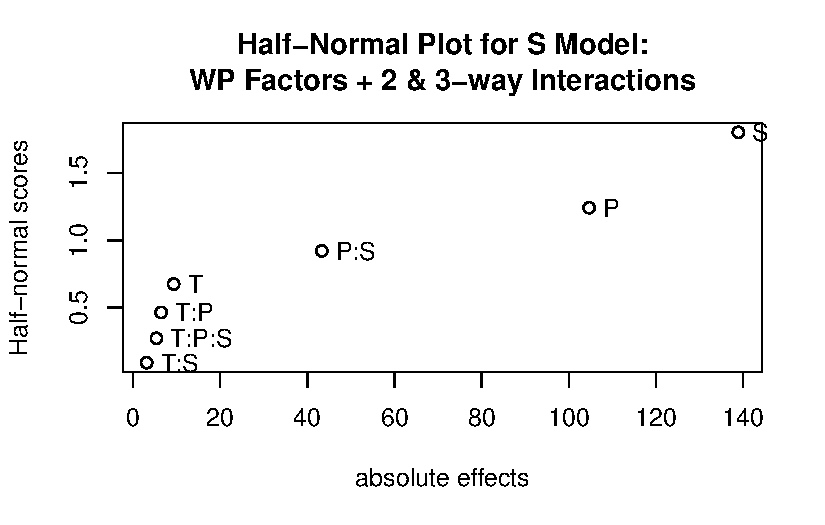
\includegraphics[keepaspectratio]{ST695_SPD_Analysis_files/figure-latex/S Model with QQ Plot-1.pdf}}

\begin{Shaded}
\begin{Highlighting}[]
\CommentTok{\# Model for SP factors and WP:SP interactions}
\NormalTok{SP\_terms }\OtherTok{\textless{}{-}} \FunctionTok{paste}\NormalTok{(}
  \StringTok{"("}\NormalTok{, }
  \FunctionTok{paste}\NormalTok{(SP\_factors, }\AttributeTok{collapse =} \StringTok{" + "}\NormalTok{), }
  \StringTok{")\^{}2"}
\NormalTok{)}

\CommentTok{\# Interactions between each WP\_factor and each SP\_factor}
\NormalTok{WP\_SP\_interactions }\OtherTok{\textless{}{-}} \FunctionTok{paste}\NormalTok{(}
  \FunctionTok{outer}\NormalTok{(}
\NormalTok{    WP\_factors,}
\NormalTok{    SP\_factors,}
    \ControlFlowTok{function}\NormalTok{(w, s) }\FunctionTok{paste}\NormalTok{(w, s, }\AttributeTok{sep =} \StringTok{":"}\NormalTok{)}
\NormalTok{  ),}
  \AttributeTok{collapse =} \StringTok{" + "}
\NormalTok{)}
\CommentTok{\# Combine into one formula string}
\NormalTok{formula\_SW }\OtherTok{\textless{}{-}} \FunctionTok{paste}\NormalTok{(}
  \StringTok{"Denier \textasciitilde{}"}\NormalTok{,}
\NormalTok{  SP\_terms,}
  \StringTok{"+"}\NormalTok{,}
\NormalTok{  WP\_SP\_interactions}
\NormalTok{)}

\CommentTok{\# If you need the split{-}plot error structure, add + Error(WP)}
\CommentTok{\# formula\_str \textless{}{-} paste(formula\_str, "+ Error(WP)")}


\NormalTok{model\_SW }\OtherTok{\textless{}{-}} \FunctionTok{lm}\NormalTok{(formula\_SW, }\AttributeTok{data =}\NormalTok{ Ys\_data)}
\NormalTok{effects\_SW }\OtherTok{\textless{}{-}} \FunctionTok{coef}\NormalTok{(model\_SW)[}\SpecialCharTok{{-}}\DecValTok{1}\NormalTok{]}
\NormalTok{effect\_names\_SW }\OtherTok{\textless{}{-}} \FunctionTok{names}\NormalTok{(}\FunctionTok{coef}\NormalTok{(model\_SW))[}\SpecialCharTok{{-}}\DecValTok{1}\NormalTok{]}

\FunctionTok{halfnormal}\NormalTok{(}
\NormalTok{  effects\_SW,}
  \AttributeTok{main =} \StringTok{"Half{-}Normal Plot for S Model :}\SpecialCharTok{\textbackslash{}n}\StringTok{SP Factors + 2{-}way Interactions +}\SpecialCharTok{\textbackslash{}n}\StringTok{ 2{-}way Interactions with WP Factors"}\NormalTok{,}
  \AttributeTok{labs =}\NormalTok{ effect\_names\_SW,}
  \AttributeTok{alpha =} \DecValTok{1}
\NormalTok{)}
\end{Highlighting}
\end{Shaded}

\begin{verbatim}
simulated critical values not available for all requests, used conservative ones
\end{verbatim}

\pandocbounded{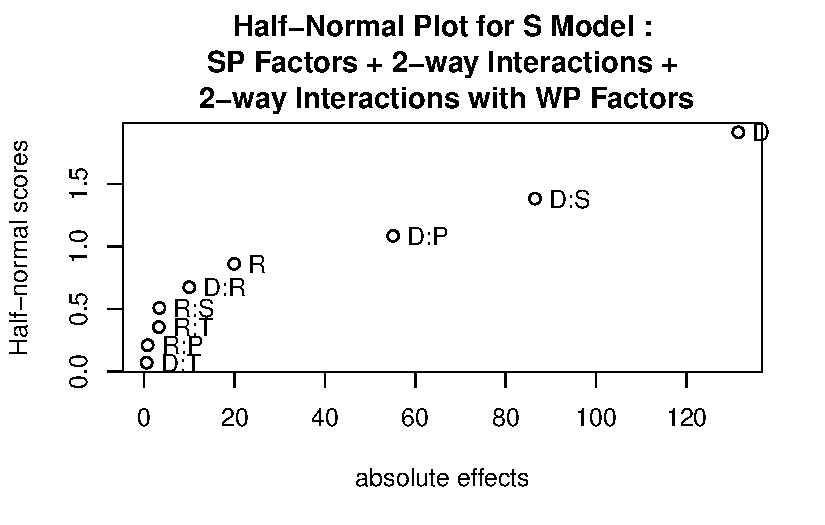
\includegraphics[keepaspectratio]{ST695_SPD_Analysis_files/figure-latex/S Model with QQ Plot-2.pdf}}

\textbf{Method 6 QQ Plot Method for W Model}

\begin{Shaded}
\begin{Highlighting}[]
\FunctionTok{library}\NormalTok{(FrF2)}

\NormalTok{WP\_factors }\OtherTok{\textless{}{-}} \FunctionTok{colnames}\NormalTok{(Ys\_data[}\DecValTok{1}\SpecialCharTok{:}\DecValTok{3}\NormalTok{])}

\CommentTok{\# Model for WP factors (main effects, 2{-} and 3{-}way interactions)}
\NormalTok{formula\_wp }\OtherTok{\textless{}{-}} \FunctionTok{as.formula}\NormalTok{(}
  \FunctionTok{paste}\NormalTok{(}
    \StringTok{"Denier \textasciitilde{} ("}\NormalTok{,}
    \FunctionTok{paste}\NormalTok{(WP\_factors, }\AttributeTok{collapse =} \StringTok{" + "}\NormalTok{),}
    \StringTok{")\^{}3"}
\NormalTok{  )}
\NormalTok{)}
                         
\NormalTok{model\_wp }\OtherTok{\textless{}{-}} \FunctionTok{lm}\NormalTok{(formula\_wp, }\AttributeTok{data =}\NormalTok{ Ys\_data)}
\NormalTok{effects\_wp }\OtherTok{\textless{}{-}} \FunctionTok{coef}\NormalTok{(model\_wp)[}\SpecialCharTok{{-}}\DecValTok{1}\NormalTok{]}
\NormalTok{effect\_names\_wp }\OtherTok{\textless{}{-}} \FunctionTok{names}\NormalTok{(}\FunctionTok{coef}\NormalTok{(model\_wp))[}\SpecialCharTok{{-}}\DecValTok{1}\NormalTok{]}

\FunctionTok{halfnormal}\NormalTok{(}
\NormalTok{  effects\_wp,}
  \AttributeTok{main =} \StringTok{"Half{-}Normal Plot for W Model:}\SpecialCharTok{\textbackslash{}n}\StringTok{WP Factors + 2 \& 3{-}way Interactions"}\NormalTok{,}
  \AttributeTok{labs =}\NormalTok{ effect\_names\_wp,}
  \AttributeTok{alpha =} \DecValTok{1}
\NormalTok{)}
\end{Highlighting}
\end{Shaded}

\begin{verbatim}
simulated critical values not available for all requests, used conservative ones
\end{verbatim}

\pandocbounded{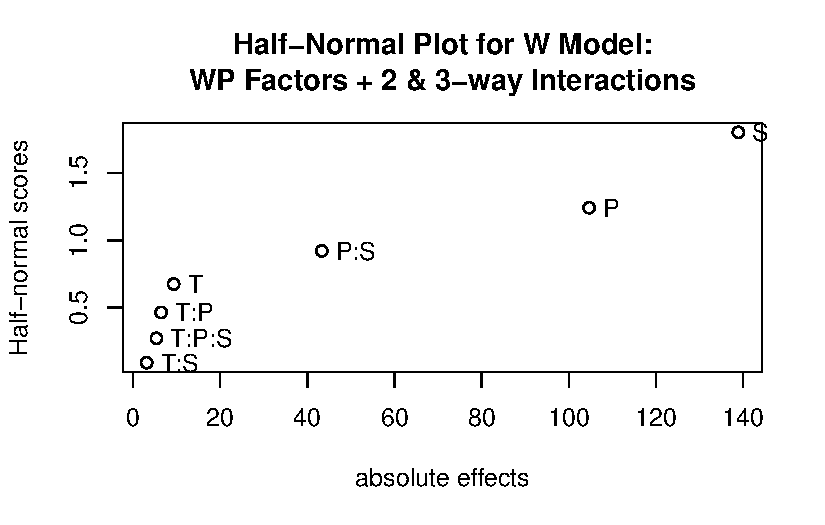
\includegraphics[keepaspectratio]{ST695_SPD_Analysis_files/figure-latex/W Model with QQ Plot-1.pdf}}

\textbf{Method 7 Lenth Method for W Model}

\begin{Shaded}
\begin{Highlighting}[]
\FunctionTok{library}\NormalTok{(BsMD)}
\end{Highlighting}
\end{Shaded}

\begin{verbatim}

Attaching package: 'BsMD'
\end{verbatim}

\begin{verbatim}
The following object is masked from 'package:FrF2':

    DanielPlot
\end{verbatim}

\begin{Shaded}
\begin{Highlighting}[]
\NormalTok{WP\_factors }\OtherTok{\textless{}{-}} \FunctionTok{colnames}\NormalTok{(Ys\_data[}\DecValTok{1}\SpecialCharTok{:}\DecValTok{3}\NormalTok{])}

\CommentTok{\# Model for WP factors (main effects, 2{-} and 3{-}way interactions)}
\NormalTok{formula\_wp }\OtherTok{\textless{}{-}} \FunctionTok{as.formula}\NormalTok{(}
  \FunctionTok{paste}\NormalTok{(}
    \StringTok{"Denier \textasciitilde{} ("}\NormalTok{,}
    \FunctionTok{paste}\NormalTok{(WP\_factors, }\AttributeTok{collapse =} \StringTok{" + "}\NormalTok{),}
    \StringTok{")\^{}3"}
\NormalTok{  )}
\NormalTok{)}

\NormalTok{model\_wp }\OtherTok{\textless{}{-}} \FunctionTok{lm}\NormalTok{(formula\_wp, }\AttributeTok{data =}\NormalTok{ Yw\_data)}
\NormalTok{effects }\OtherTok{\textless{}{-}} \FunctionTok{coef}\NormalTok{(model\_wp)[}\SpecialCharTok{{-}}\DecValTok{1}\NormalTok{]  }\CommentTok{\# Remove intercept}
\FunctionTok{LenthPlot}\NormalTok{(effects, }\AttributeTok{main =} \StringTok{"Lenth Plot for W Model: All Effects"}\NormalTok{)}
\end{Highlighting}
\end{Shaded}

\pandocbounded{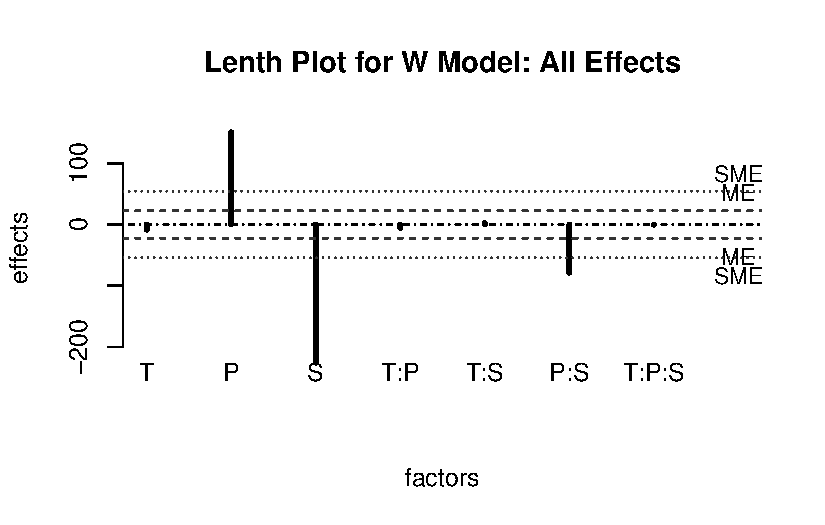
\includegraphics[keepaspectratio]{ST695_SPD_Analysis_files/figure-latex/W Model by Lenth Method-1.pdf}}

\begin{verbatim}
   alpha      PSE       ME      SME 
 0.05000  6.01875 22.65532 54.21875 
\end{verbatim}

\textbf{Method 8 Sequential Split Plot Method for W Model}

\begin{Shaded}
\begin{Highlighting}[]
\NormalTok{WP\_factors }\OtherTok{\textless{}{-}} \FunctionTok{colnames}\NormalTok{(Yw\_data[}\DecValTok{1}\SpecialCharTok{:}\DecValTok{3}\NormalTok{])}


\CommentTok{\# Model for WP factors (main effects, 2{-}way interactions)}
\NormalTok{formula\_wp }\OtherTok{\textless{}{-}} \FunctionTok{as.formula}\NormalTok{(}
  \FunctionTok{paste}\NormalTok{(}
    \StringTok{"Denier \textasciitilde{} ("}\NormalTok{,}
    \FunctionTok{paste}\NormalTok{(WP\_factors, }\AttributeTok{collapse =} \StringTok{" + "}\NormalTok{),}
    \StringTok{")\^{}2"}
\NormalTok{  )}
\NormalTok{)}

\NormalTok{Method\_8 }\OtherTok{\textless{}{-}} \FunctionTok{summary}\NormalTok{(}\FunctionTok{lm}\NormalTok{(formula\_wp, }\AttributeTok{data =}\NormalTok{ Yw\_data))}

\NormalTok{Method\_8}
\end{Highlighting}
\end{Shaded}

\begin{verbatim}

Call:
lm.default(formula = formula_wp, data = Yw_data)

Residuals:
      1       2       3       4       5       6       7       8 
 0.5125 -0.5125 -0.5125  0.5125 -0.5125  0.5125  0.5125 -0.5125 

Coefficients:
             Estimate Std. Error  t value Pr(>|t|)    
(Intercept)  443.4875     0.5125  865.341 0.000736 ***
T             -8.5375     0.5125  -16.659 0.038170 *  
P            150.6625     0.5125  293.976 0.002166 ** 
S           -225.7625     0.5125 -440.512 0.001445 ** 
T:P           -5.7125     0.5125  -11.146 0.056962 .  
T:S            2.3125     0.5125    4.512 0.138845    
P:S          -78.7375     0.5125 -153.634 0.004144 ** 
---
Signif. codes:  0 '***' 0.001 '**' 0.01 '*' 0.05 '.' 0.1 ' ' 1

Residual standard error: 1.45 on 1 degrees of freedom
Multiple R-squared:      1, Adjusted R-squared:      1 
F-statistic: 5.075e+04 on 6 and 1 DF,  p-value: 0.003398
\end{verbatim}




\end{document}
